\documentclass[tikz,border=2pt]{standalone}
\usepackage{amsmath,amssymb,fix-cm}
\usetikzlibrary{arrows.meta,positioning,shapes.geometric}
\begin{document}
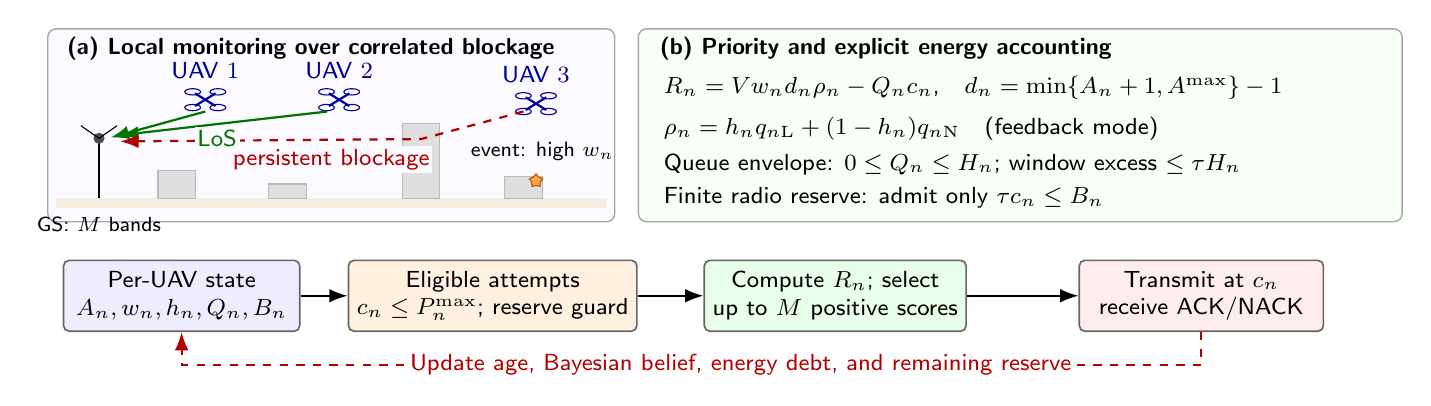
\begin{tikzpicture}[font=\sffamily\fontsize{8.4}{10}\selectfont,>={Latex[length=2mm]},
 panel/.style={rounded corners=3pt,draw=black!35,line width=.5pt},
 block/.style={rounded corners=2pt,draw=black!60,line width=.6pt,align=center,minimum height=9mm,inner sep=3pt},
 arrow/.style={-Latex,line width=.8pt}]
\draw[panel,fill=blue!2] (0,0) rectangle (7.2,2.45);
\node[anchor=west,font=\sffamily\bfseries\fontsize{8.4}{10}\selectfont] at (.12,2.20){(a) Local monitoring over correlated blockage};
\fill[brown!15] (.1,.18) rectangle (7.1,.30);
\foreach \x/\h in {1.4/.65,2.8/.48,4.5/1.25,5.8/.58}{\fill[gray!25,draw=gray!55] (\x,.30) rectangle (\x+.48,\h);}
\draw[line width=1pt] (.65,.30)--(.65,1.02);
\fill[black!70] (.65,1.06) circle (2pt);
\draw (.42,1.22)--(.65,1.06)--(.88,1.22);
\node[anchor=north,font=\sffamily\fontsize{7.4}{9}\selectfont] at (.65,.18){GS: $M$ bands};
\foreach \x/\y/\label in {2/1.55/1,3.7/1.55/2,6.2/1.50/3}{
 \draw[blue!60!black,line width=.8pt] (\x-.13,\y-.08)--(\x+.13,\y+.08) (\x-.13,\y+.08)--(\x+.13,\y-.08);
 \foreach \dx/\dy in {-.16/-.10,-.16/.10,.16/-.10,.16/.10}{\draw[blue!60!black] (\x+\dx,\y+\dy) ellipse (.10 and .04);}
 \node[anchor=south,blue!60!black] at (\x,\y+.14){UAV $\label$};}
\draw[arrow,green!45!black] (2,1.40)--(.80,1.07);
\draw[arrow,green!45!black] (3.55,1.40)--(.92,1.10);
\draw[arrow,red!70!black,dashed] (6.04,1.40)--(4.74,1.05)--(.92,1.02);
\node[green!45!black,fill=blue!2,inner sep=1pt] at (2.15,1.06){LoS};
\node[red!70!black,fill=blue!2,inner sep=1pt] at (3.6,.79){persistent blockage};
\node[star,star points=5,fill=orange!70,draw=orange!70!black,minimum size=5pt,inner sep=0pt] at (6.2,.52){};
\node[anchor=west,font=\sffamily\fontsize{7.5}{9}\selectfont] at (5.25,.89){event: high $w_n$};
\draw[panel,fill=green!3] (7.5,0) rectangle (17.2,2.45);
\node[anchor=west,font=\sffamily\bfseries\fontsize{8.4}{10}\selectfont] at (7.65,2.20){(b) Priority and explicit energy accounting};
\node[anchor=west] at (7.7,1.70){$R_n=Vw_nd_n\rho_n-Q_nc_n$,\quad $d_n=\min\{A_n+1,A^{\max}\}-1$};
\node[anchor=west] at (7.7,1.18){$\rho_n=h_nq_{n\mathrm L}+(1-h_n)q_{n\mathrm N}$\quad (feedback mode)};
\node[anchor=west] at (7.7,.73){Queue envelope: $0\le Q_n\le H_n$; window excess $\le\tau H_n$};
\node[anchor=west] at (7.7,.30){Finite radio reserve: admit only $\tau c_n\le B_n$};
\node[block,fill=blue!7,minimum width=30mm] (state) at (1.7,-.94){Per-UAV state\\$A_n,w_n,h_n,Q_n,B_n$};
\node[block,fill=orange!12,minimum width=30mm] (guard) at (5.65,-.94){Eligible attempts\\$c_n\le P_n^{\max}$; reserve guard};
\node[block,fill=green!9,minimum width=31mm] (select) at (10.00,-.94){Compute $R_n$; select\\up to $M$ positive scores};
\node[block,fill=red!7,minimum width=31mm] (tx) at (14.65,-.94){Transmit at $c_n$\\receive ACK/NACK};
\draw[arrow] (state)--(guard);\draw[arrow] (guard)--(select);\draw[arrow] (select)--(tx);
\draw[arrow,dashed,red!70!black] (tx.south)--(14.65,-1.82)--(1.7,-1.82)--(state.south);
\node[fill=white,inner sep=1pt,text=red!70!black] at (8.8,-1.82){Update age, Bayesian belief, energy debt, and remaining reserve};
\end{tikzpicture}
\end{document}
